% Options for packages loaded elsewhere
\PassOptionsToPackage{unicode}{hyperref}
\PassOptionsToPackage{hyphens}{url}
%
\documentclass[
]{article}
\usepackage{lmodern}
\usepackage{amssymb,amsmath}
\usepackage{ifxetex,ifluatex}
\ifnum 0\ifxetex 1\fi\ifluatex 1\fi=0 % if pdftex
  \usepackage[T1]{fontenc}
  \usepackage[utf8]{inputenc}
  \usepackage{textcomp} % provide euro and other symbols
\else % if luatex or xetex
  \usepackage{unicode-math}
  \defaultfontfeatures{Scale=MatchLowercase}
  \defaultfontfeatures[\rmfamily]{Ligatures=TeX,Scale=1}
\fi
% Use upquote if available, for straight quotes in verbatim environments
\IfFileExists{upquote.sty}{\usepackage{upquote}}{}
\IfFileExists{microtype.sty}{% use microtype if available
  \usepackage[]{microtype}
  \UseMicrotypeSet[protrusion]{basicmath} % disable protrusion for tt fonts
}{}
\makeatletter
\@ifundefined{KOMAClassName}{% if non-KOMA class
  \IfFileExists{parskip.sty}{%
    \usepackage{parskip}
  }{% else
    \setlength{\parindent}{0pt}
    \setlength{\parskip}{6pt plus 2pt minus 1pt}}
}{% if KOMA class
  \KOMAoptions{parskip=half}}
\makeatother
\usepackage{xcolor}
\IfFileExists{xurl.sty}{\usepackage{xurl}}{} % add URL line breaks if available
\IfFileExists{bookmark.sty}{\usepackage{bookmark}}{\usepackage{hyperref}}
\hypersetup{
  pdftitle={Do global oil price movements offer insight into the performance of the South African Rand?},
  pdfauthor={Tangeni Shatiwa},
  hidelinks,
  pdfcreator={LaTeX via pandoc}}
\urlstyle{same} % disable monospaced font for URLs
\usepackage[margin=1in]{geometry}
\usepackage{graphicx,grffile}
\makeatletter
\def\maxwidth{\ifdim\Gin@nat@width>\linewidth\linewidth\else\Gin@nat@width\fi}
\def\maxheight{\ifdim\Gin@nat@height>\textheight\textheight\else\Gin@nat@height\fi}
\makeatother
% Scale images if necessary, so that they will not overflow the page
% margins by default, and it is still possible to overwrite the defaults
% using explicit options in \includegraphics[width, height, ...]{}
\setkeys{Gin}{width=\maxwidth,height=\maxheight,keepaspectratio}
% Set default figure placement to htbp
\makeatletter
\def\fps@figure{htbp}
\makeatother
\setlength{\emergencystretch}{3em} % prevent overfull lines
\providecommand{\tightlist}{%
  \setlength{\itemsep}{0pt}\setlength{\parskip}{0pt}}
\setcounter{secnumdepth}{-\maxdimen} % remove section numbering

\title{Do global oil price movements offer insight into the performance of the
South African Rand?}
\author{Tangeni Shatiwa}
\date{2020-06-11T21:13:14-05:00}

\begin{document}
\maketitle

\emph{For much of the past decade, the South African Rand has been
regarded to be amongst the most volatile currencies in the world.
However, nothing from the past 10 years could have prepared Rand
investors for the set of unprecedented events which 2020 has brought so
far. Essentially, the South African economy has been hit by a perfect
storm following a series of sovereign credit rating downgrades in April
by Moody's and S\&P, compounded even further by the COVID-19 pandemic.
This resulted in a huge Rand sell-off equating to roughly 28\% against
the dollar between January and April 2020, as the USD-ZAR reached an all
time low of R19.35. Since then, the Rand has partially clawed back from
this slump as the world begins to re-emerge from national lockdowns
imposed to curb the spread of the pandemic.}

\emph{Given South Africa's exposure to oil prices (particularly with
Brent crude oil being priced in dollars), directional movements of oil
prices can be an extremely useful tool in analyzing the USD-ZAR exchange
rate. Oil-Rand analyses hold merit on the premise that oil price
movements offer a snapshot of the global dynamics of which the Rand is
also exposed to.}

\hypertarget{the-dynamics-of-oil-prices-as-a-measure-for-rand-performance}{%
\subsection{The dynamics of oil prices as a measure for Rand
performance}\label{the-dynamics-of-oil-prices-as-a-measure-for-rand-performance}}

In theory, lower global oil prices are supposed to have a positive
effect on the Rand (through an improved trade balance), given that South
Africa imports its oil. Although it is plausible that this relationship
exists when taking a long-term view on the South African economy, it is
interesting to find that the exact opposite effect tends to persist
through the short-run. Rand weakening tends to coincide with periods in
which global oil prices are on the decline, and vice versa.

There are several reasons which explain why the abovementioned
phenomenon exists. Firstly, the value of both of these commodities are
likely to fall simultaneously during periods of global risk aversion, as
investors ditch risky assets in favor of safe-haven ones (such as the
USD). Secondly, lower global oil prices could be a reflection that
global growth (and commodity prices in a broad sense) are on the
decline, which would adversely impact the value of commodity-linked
currencies (the Rand in this case). Finally, because global oil prices
are denominated in USD, declining oil prices in dollar terms would
indicate that the greenback currency has strengthened, which by symmetry
implies a weakened Rand.

These sentiments are supported by trends identified in Figure
@ref(fig:scatter). Notably, stronger Rand levels (i.e a lower USD-ZAR
exchange rate) occur more frequently when oil prices are trading at
higher levels. Interestingly, lower oil prices (and a weaker Rand)
generally coincide with periods of high market uncertainty. In order to
quantify these periods of market uncertainty, one can use the CBOE
Volatility Index (VIX).\footnote{The CBOE VIX measures the market's
  expectation of 30-day forward-looking volatility on S\&P 500 Options.
  This index is commonly used in financial analysis as a proxy for
  global market uncertainty.} From this, it is evident that higher
levels of volatility (illustrated by the darker observations from the
distribution of outcomes in Figure @ref(fig:scatter)) are increasingly
prevalent when the oil price trades below the USD40 per barrel mark.
Clearly, the trend line in Figure @ref(fig:scatter) also indicates that
there is a non-linear relationship between the oil price and the Rand.
This means that the further the oil price declines, the sharper the
depreciation in the Rand would be (i.e depreciating at an increasing
rate). This is exactly what we have seen between February and April,
which underpins just how important risk sentiment is when predicting the
path for a commodity-linked currency such as the Rand.

\begin{figure}
\centering
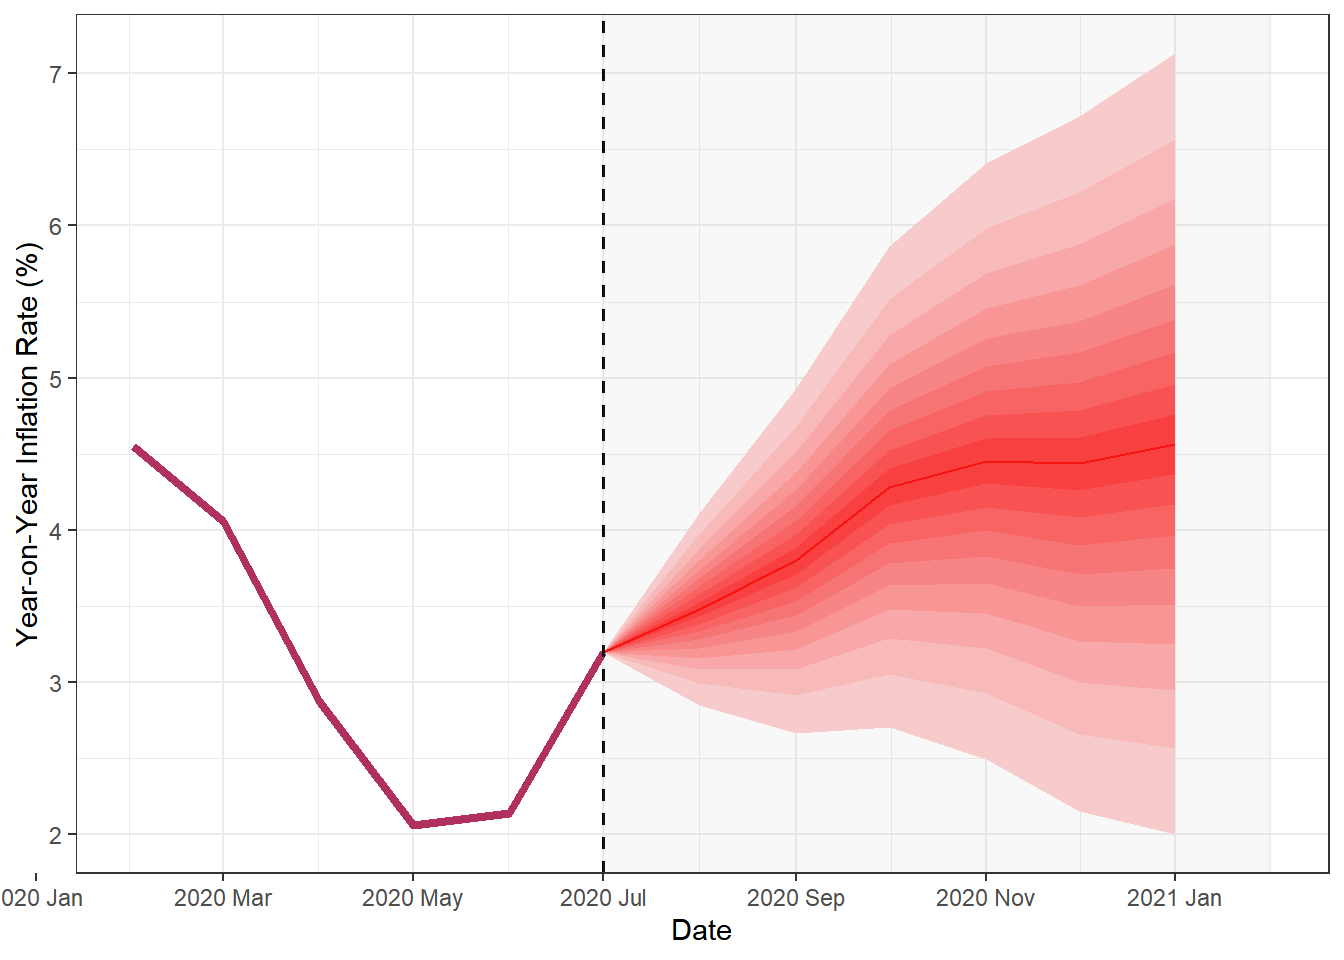
\includegraphics{2020-06-11_files/figure-latex/scatter-1.pdf}
\caption{Weekly data downloaded from Yahoo Finance (Jan 2015-June
2020).}
\end{figure}

\hypertarget{this-model-suggests-that-given-current-oil-price-levels-the-rand-is-undervalued}{%
\subsection{This model suggests that given current oil price levels, the
Rand is
undervalued}\label{this-model-suggests-that-given-current-oil-price-levels-the-rand-is-undervalued}}

As of the 10\textsuperscript{th} of June, Brent crude oil and the Rand
were trading at actual levels of around USD38 per barrel and R16.50
(against the USD) respectively. We can derive an implied value for the
Rand by analyzing the non-linear trend line in Figure @ref(fig:scatter).
With this, a USD38 price level for a barrel of crude oil implies that
the Rand should be trading closer to R15.50, which suggests that the
Rand is undervalued at the moment. This is encouraging - an undervalued
view on the Rand could bode well for its outlook over the near-to-mid
term, as foreign and local investors continue their search for
high-yield investment opportunities. This bullish view on the local
currency is supported further by the following considerations

\begin{itemize}
\tightlist
\item
  A recovery in oil prices following the unprecedented sell-offs between
  February and April. This is set to be fuelled by 1) an improvement in
  global oil demand as countries transition out of periods of lockdown,
  as well as 2) supply-side stimulus effects on the back of the historic
  OPEC+ agreement reached in early April.
\item
  A low/zero interest rate environment throughout Europe and the US,
  which has recently seen investors being squeezed towards buying
  riskier assets (such as the Rand).
\item
  South African bond liquidations have eased in recent weeks when
  contrasted with the rapid rate at which investors were dumping these
  bonds in the build-up to Moody's sovereign credit rating decision in
  April.
\item
  A bullish view on gold prices should provide some relief for South
  Africa's exports and trade balance, which would theoretically boost
  the Rand (South Africa is a major gold producer).
\end{itemize}

Of course, there are notable downside risks which oil prices and
emerging market currencies are faced with in the current economic
landscape. For one, a second wave of the COVID-19 pandemic in countries
that have managed to slow the initial transmission of the virus could
re-trigger a spike in market uncertainty, similar to what we experienced
earlier this year. Also, an escalation in market uncertainty could be
exacerbated by heightened trade tensions between the US and China, which
would force investors to be bearish towards the Rand. Lastly, it is no
secret that South African economic prospects continue to be hampered by
poor growth levels and a deterioration in public debt. Therefore, it
remains to be seen whether these headwinds will outweigh the prospects
for a further recovery in the Rand over the next few months. Without a
shadow of a doubt, investors and the general South African public will
be monitoring these developments quite closely.

\end{document}
